% Created by tikzDevice version 0.12.3 on 2020-06-04 22:28:42
% !TEX encoding = UTF-8 Unicode
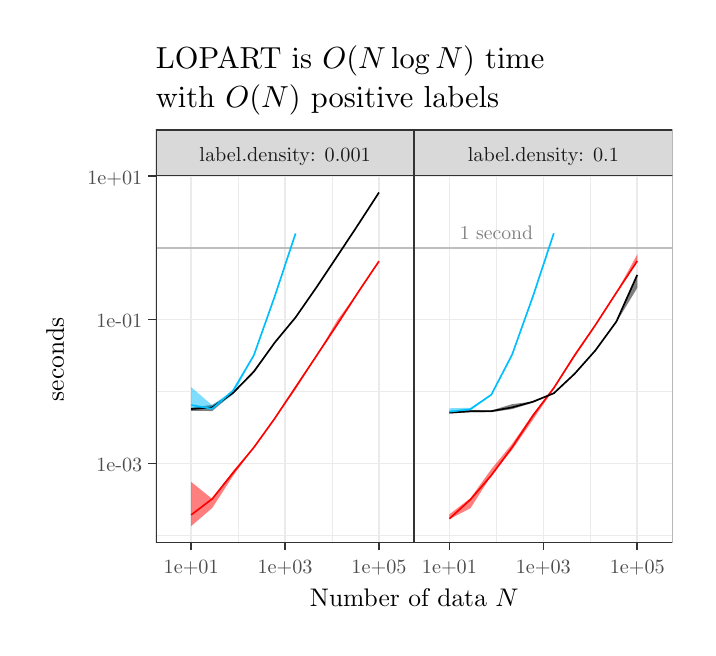
\begin{tikzpicture}[x=1pt,y=1pt]
\definecolor{fillColor}{RGB}{255,255,255}
\path[use as bounding box,fill=fillColor,fill opacity=0.00] (0,0) rectangle (238.49,216.81);
\begin{scope}
\path[clip] (  0.00,  0.00) rectangle (238.49,216.81);
\definecolor{drawColor}{RGB}{255,255,255}
\definecolor{fillColor}{RGB}{255,255,255}

\path[draw=drawColor,line width= 0.6pt,line join=round,line cap=round,fill=fillColor] (  0.00,  0.00) rectangle (238.49,216.81);
\end{scope}
\begin{scope}
\path[clip] ( 46.36, 30.69) rectangle (139.68,163.33);
\definecolor{fillColor}{RGB}{255,255,255}

\path[fill=fillColor] ( 46.36, 30.69) rectangle (139.68,163.33);
\definecolor{drawColor}{gray}{0.92}

\path[draw=drawColor,line width= 0.3pt,line join=round] ( 46.36, 33.41) --
	(139.68, 33.41);

\path[draw=drawColor,line width= 0.3pt,line join=round] ( 46.36, 85.35) --
	(139.68, 85.35);

\path[draw=drawColor,line width= 0.3pt,line join=round] ( 46.36,137.29) --
	(139.68,137.29);

\path[draw=drawColor,line width= 0.3pt,line join=round] ( 76.06, 30.69) --
	( 76.06,163.33);

\path[draw=drawColor,line width= 0.3pt,line join=round] (109.99, 30.69) --
	(109.99,163.33);

\path[draw=drawColor,line width= 0.6pt,line join=round] ( 46.36, 59.38) --
	(139.68, 59.38);

\path[draw=drawColor,line width= 0.6pt,line join=round] ( 46.36,111.32) --
	(139.68,111.32);

\path[draw=drawColor,line width= 0.6pt,line join=round] ( 46.36,163.26) --
	(139.68,163.26);

\path[draw=drawColor,line width= 0.6pt,line join=round] ( 59.09, 30.69) --
	( 59.09,163.33);

\path[draw=drawColor,line width= 0.6pt,line join=round] ( 93.02, 30.69) --
	( 93.02,163.33);

\path[draw=drawColor,line width= 0.6pt,line join=round] (126.95, 30.69) --
	(126.95,163.33);
\definecolor{drawColor}{RGB}{190,190,190}

\path[draw=drawColor,line width= 0.6pt,line join=round] ( 46.36,137.29) -- (139.68,137.29);
\definecolor{fillColor}{RGB}{255,0,0}

\path[fill=fillColor,fill opacity=0.50] ( 59.09, 52.65) --
	( 66.68, 46.53) --
	( 74.22, 56.61) --
	( 81.73, 65.18) --
	( 89.26, 75.82) --
	( 96.80, 86.94) --
	(104.33, 98.20) --
	(111.87,111.09) --
	(119.41,121.28) --
	(126.95,132.64) --
	(126.95,132.37) --
	(119.41,120.85) --
	(111.87,109.53) --
	(104.33, 98.03) --
	( 96.80, 86.08) --
	( 89.26, 75.54) --
	( 81.73, 65.09) --
	( 74.22, 54.88) --
	( 66.68, 43.24) --
	( 59.09, 36.71) --
	cycle;

\path[] ( 59.09, 52.65) --
	( 66.68, 46.53) --
	( 74.22, 56.61) --
	( 81.73, 65.18) --
	( 89.26, 75.82) --
	( 96.80, 86.94) --
	(104.33, 98.20) --
	(111.87,111.09) --
	(119.41,121.28) --
	(126.95,132.64);

\path[] (126.95,132.37) --
	(119.41,120.85) --
	(111.87,109.53) --
	(104.33, 98.03) --
	( 96.80, 86.08) --
	( 89.26, 75.54) --
	( 81.73, 65.09) --
	( 74.22, 54.88) --
	( 66.68, 43.24) --
	( 59.09, 36.71);
\definecolor{fillColor}{RGB}{0,0,0}

\path[fill=fillColor,fill opacity=0.50] ( 59.09, 79.51) --
	( 66.68, 80.51) --
	( 74.22, 84.87) --
	( 81.73, 93.02) --
	( 89.26,103.01) --
	( 96.80,112.19) --
	(104.33,122.96) --
	(111.87,134.56) --
	(119.41,145.72) --
	(126.95,157.30) --
	(126.95,157.17) --
	(119.41,145.62) --
	(111.87,134.17) --
	(104.33,122.94) --
	( 96.80,111.98) --
	( 89.26,102.82) --
	( 81.73, 92.38) --
	( 74.22, 84.63) --
	( 66.68, 78.28) --
	( 59.09, 78.36) --
	cycle;

\path[] ( 59.09, 79.51) --
	( 66.68, 80.51) --
	( 74.22, 84.87) --
	( 81.73, 93.02) --
	( 89.26,103.01) --
	( 96.80,112.19) --
	(104.33,122.96) --
	(111.87,134.56) --
	(119.41,145.72) --
	(126.95,157.30);

\path[] (126.95,157.17) --
	(119.41,145.62) --
	(111.87,134.17) --
	(104.33,122.94) --
	( 96.80,111.98) --
	( 89.26,102.82) --
	( 81.73, 92.38) --
	( 74.22, 84.63) --
	( 66.68, 78.28) --
	( 59.09, 78.36);
\definecolor{fillColor}{RGB}{0,191,255}

\path[fill=fillColor,fill opacity=0.50] ( 59.09, 86.91) --
	( 66.68, 80.35) --
	( 74.22, 85.81) --
	( 81.73, 98.65) --
	( 89.26,119.77) --
	( 96.80,142.45) --
	( 96.80,142.39) --
	( 89.26,119.65) --
	( 81.73, 98.34) --
	( 74.22, 84.16) --
	( 66.68, 78.89) --
	( 59.09, 79.24) --
	cycle;

\path[] ( 59.09, 86.91) --
	( 66.68, 80.35) --
	( 74.22, 85.81) --
	( 81.73, 98.65) --
	( 89.26,119.77) --
	( 96.80,142.45);

\path[] ( 96.80,142.39) --
	( 89.26,119.65) --
	( 81.73, 98.34) --
	( 74.22, 84.16) --
	( 66.68, 78.89) --
	( 59.09, 79.24);
\definecolor{drawColor}{RGB}{255,0,0}

\path[draw=drawColor,line width= 0.6pt,line join=round] ( 59.09, 40.76) --
	( 66.68, 46.53) --
	( 74.22, 55.97) --
	( 81.73, 65.12) --
	( 89.26, 75.57) --
	( 96.80, 86.90) --
	(104.33, 98.20) --
	(111.87,109.59) --
	(119.41,121.22) --
	(126.95,132.43);
\definecolor{drawColor}{RGB}{0,0,0}

\path[draw=drawColor,line width= 0.6pt,line join=round] ( 59.09, 79.00) --
	( 66.68, 79.58) --
	( 74.22, 84.85) --
	( 81.73, 92.50) --
	( 89.26,103.00) --
	( 96.80,112.11) --
	(104.33,122.95) --
	(111.87,134.23) --
	(119.41,145.63) --
	(126.95,157.27);
\definecolor{drawColor}{RGB}{0,191,255}

\path[draw=drawColor,line width= 0.6pt,line join=round] ( 59.09, 80.44) --
	( 66.68, 79.08) --
	( 74.22, 85.67) --
	( 81.73, 98.43) --
	( 89.26,119.68) --
	( 96.80,142.44);
\definecolor{drawColor}{gray}{0.20}

\path[draw=drawColor,line width= 0.6pt,line join=round,line cap=round] ( 46.36, 30.69) rectangle (139.68,163.33);
\end{scope}
\begin{scope}
\path[clip] (139.68, 30.69) rectangle (232.99,163.33);
\definecolor{fillColor}{RGB}{255,255,255}

\path[fill=fillColor] (139.68, 30.69) rectangle (232.99,163.33);
\definecolor{drawColor}{gray}{0.92}

\path[draw=drawColor,line width= 0.3pt,line join=round] (139.68, 33.41) --
	(232.99, 33.41);

\path[draw=drawColor,line width= 0.3pt,line join=round] (139.68, 85.35) --
	(232.99, 85.35);

\path[draw=drawColor,line width= 0.3pt,line join=round] (139.68,137.29) --
	(232.99,137.29);

\path[draw=drawColor,line width= 0.3pt,line join=round] (169.37, 30.69) --
	(169.37,163.33);

\path[draw=drawColor,line width= 0.3pt,line join=round] (203.30, 30.69) --
	(203.30,163.33);

\path[draw=drawColor,line width= 0.6pt,line join=round] (139.68, 59.38) --
	(232.99, 59.38);

\path[draw=drawColor,line width= 0.6pt,line join=round] (139.68,111.32) --
	(232.99,111.32);

\path[draw=drawColor,line width= 0.6pt,line join=round] (139.68,163.26) --
	(232.99,163.26);

\path[draw=drawColor,line width= 0.6pt,line join=round] (152.40, 30.69) --
	(152.40,163.33);

\path[draw=drawColor,line width= 0.6pt,line join=round] (186.33, 30.69) --
	(186.33,163.33);

\path[draw=drawColor,line width= 0.6pt,line join=round] (220.27, 30.69) --
	(220.27,163.33);
\definecolor{drawColor}{RGB}{190,190,190}

\path[draw=drawColor,line width= 0.6pt,line join=round] (139.68,137.29) -- (232.99,137.29);
\definecolor{drawColor}{gray}{0.50}

\node[text=drawColor,anchor=base,inner sep=0pt, outer sep=0pt, scale=  0.71] at (169.37,140.23) {1 second};
\definecolor{fillColor}{RGB}{255,0,0}

\path[fill=fillColor,fill opacity=0.50] (152.40, 40.97) --
	(159.99, 46.79) --
	(167.54, 57.28) --
	(175.04, 66.40) --
	(182.57, 77.09) --
	(190.11, 86.88) --
	(197.65, 99.02) --
	(205.19,109.60) --
	(212.73,121.19) --
	(220.27,134.88) --
	(220.27,132.50) --
	(212.73,120.84) --
	(205.19,109.38) --
	(197.65, 98.19) --
	(190.11, 86.36) --
	(182.57, 75.11) --
	(175.04, 64.28) --
	(167.54, 54.96) --
	(159.99, 43.16) --
	(152.40, 39.24) --
	cycle;

\path[] (152.40, 40.97) --
	(159.99, 46.79) --
	(167.54, 57.28) --
	(175.04, 66.40) --
	(182.57, 77.09) --
	(190.11, 86.88) --
	(197.65, 99.02) --
	(205.19,109.60) --
	(212.73,121.19) --
	(220.27,134.88);

\path[] (220.27,132.50) --
	(212.73,120.84) --
	(205.19,109.38) --
	(197.65, 98.19) --
	(190.11, 86.36) --
	(182.57, 75.11) --
	(175.04, 64.28) --
	(167.54, 54.96) --
	(159.99, 43.16) --
	(152.40, 39.24);
\definecolor{fillColor}{RGB}{0,0,0}

\path[fill=fillColor,fill opacity=0.50] (152.40, 78.29) --
	(159.99, 78.65) --
	(167.54, 78.46) --
	(175.04, 80.76) --
	(182.57, 81.67) --
	(190.11, 84.81) --
	(197.65, 91.82) --
	(205.19,100.36) --
	(212.73,110.75) --
	(220.27,127.51) --
	(220.27,122.78) --
	(212.73,110.32) --
	(205.19,100.11) --
	(197.65, 91.48) --
	(190.11, 84.62) --
	(182.57, 81.26) --
	(175.04, 78.98) --
	(167.54, 77.85) --
	(159.99, 77.86) --
	(152.40, 77.38) --
	cycle;

\path[] (152.40, 78.29) --
	(159.99, 78.65) --
	(167.54, 78.46) --
	(175.04, 80.76) --
	(182.57, 81.67) --
	(190.11, 84.81) --
	(197.65, 91.82) --
	(205.19,100.36) --
	(212.73,110.75) --
	(220.27,127.51);

\path[] (220.27,122.78) --
	(212.73,110.32) --
	(205.19,100.11) --
	(197.65, 91.48) --
	(190.11, 84.62) --
	(182.57, 81.26) --
	(175.04, 78.98) --
	(167.54, 77.85) --
	(159.99, 77.86) --
	(152.40, 77.38);
\definecolor{fillColor}{RGB}{0,191,255}

\path[fill=fillColor,fill opacity=0.50] (152.40, 79.27) --
	(159.99, 79.47) --
	(167.54, 84.47) --
	(175.04, 98.74) --
	(182.57,120.29) --
	(190.11,142.51) --
	(190.11,142.35) --
	(182.57,119.64) --
	(175.04, 98.37) --
	(167.54, 84.06) --
	(159.99, 78.76) --
	(152.40, 77.78) --
	cycle;

\path[] (152.40, 79.27) --
	(159.99, 79.47) --
	(167.54, 84.47) --
	(175.04, 98.74) --
	(182.57,120.29) --
	(190.11,142.51);

\path[] (190.11,142.35) --
	(182.57,119.64) --
	(175.04, 98.37) --
	(167.54, 84.06) --
	(159.99, 78.76) --
	(152.40, 77.78);
\definecolor{drawColor}{RGB}{255,0,0}

\path[draw=drawColor,line width= 0.6pt,line join=round] (152.40, 39.38) --
	(159.99, 46.29) --
	(167.54, 55.05) --
	(175.04, 65.16) --
	(182.57, 76.65) --
	(190.11, 86.58) --
	(197.65, 98.39) --
	(205.19,109.42) --
	(212.73,121.07) --
	(220.27,132.51);
\definecolor{drawColor}{RGB}{0,0,0}

\path[draw=drawColor,line width= 0.6pt,line join=round] (152.40, 77.70) --
	(159.99, 78.19) --
	(167.54, 78.25) --
	(175.04, 79.59) --
	(182.57, 81.65) --
	(190.11, 84.69) --
	(197.65, 91.75) --
	(205.19,100.24) --
	(212.73,110.61) --
	(220.27,127.47);
\definecolor{drawColor}{RGB}{0,191,255}

\path[draw=drawColor,line width= 0.6pt,line join=round] (152.40, 78.05) --
	(159.99, 78.92) --
	(167.54, 84.18) --
	(175.04, 98.64) --
	(182.57,119.68) --
	(190.11,142.50);
\definecolor{drawColor}{gray}{0.20}

\path[draw=drawColor,line width= 0.6pt,line join=round,line cap=round] (139.68, 30.69) rectangle (232.99,163.33);
\end{scope}
\begin{scope}
\path[clip] ( 46.36,163.33) rectangle (139.68,179.90);
\definecolor{drawColor}{gray}{0.20}
\definecolor{fillColor}{gray}{0.85}

\path[draw=drawColor,line width= 0.6pt,line join=round,line cap=round,fill=fillColor] ( 46.36,163.33) rectangle (139.68,179.90);
\definecolor{drawColor}{gray}{0.10}

\node[text=drawColor,anchor=base,inner sep=0pt, outer sep=0pt, scale=  0.73] at ( 93.02,168.58) {label.density: 0.001};
\end{scope}
\begin{scope}
\path[clip] (139.68,163.33) rectangle (232.99,179.90);
\definecolor{drawColor}{gray}{0.20}
\definecolor{fillColor}{gray}{0.85}

\path[draw=drawColor,line width= 0.6pt,line join=round,line cap=round,fill=fillColor] (139.68,163.33) rectangle (232.99,179.90);
\definecolor{drawColor}{gray}{0.10}

\node[text=drawColor,anchor=base,inner sep=0pt, outer sep=0pt, scale=  0.73] at (186.33,168.58) {label.density: 0.1};
\end{scope}
\begin{scope}
\path[clip] (  0.00,  0.00) rectangle (238.49,216.81);
\definecolor{drawColor}{gray}{0.20}

\path[draw=drawColor,line width= 0.6pt,line join=round] ( 59.09, 27.94) --
	( 59.09, 30.69);

\path[draw=drawColor,line width= 0.6pt,line join=round] ( 93.02, 27.94) --
	( 93.02, 30.69);

\path[draw=drawColor,line width= 0.6pt,line join=round] (126.95, 27.94) --
	(126.95, 30.69);
\end{scope}
\begin{scope}
\path[clip] (  0.00,  0.00) rectangle (238.49,216.81);
\definecolor{drawColor}{gray}{0.30}

\node[text=drawColor,anchor=base,inner sep=0pt, outer sep=0pt, scale=  0.73] at ( 59.09, 19.68) {1e+01};

\node[text=drawColor,anchor=base,inner sep=0pt, outer sep=0pt, scale=  0.73] at ( 93.02, 19.68) {1e+03};

\node[text=drawColor,anchor=base,inner sep=0pt, outer sep=0pt, scale=  0.73] at (126.95, 19.68) {1e+05};
\end{scope}
\begin{scope}
\path[clip] (  0.00,  0.00) rectangle (238.49,216.81);
\definecolor{drawColor}{gray}{0.20}

\path[draw=drawColor,line width= 0.6pt,line join=round] (152.40, 27.94) --
	(152.40, 30.69);

\path[draw=drawColor,line width= 0.6pt,line join=round] (186.33, 27.94) --
	(186.33, 30.69);

\path[draw=drawColor,line width= 0.6pt,line join=round] (220.27, 27.94) --
	(220.27, 30.69);
\end{scope}
\begin{scope}
\path[clip] (  0.00,  0.00) rectangle (238.49,216.81);
\definecolor{drawColor}{gray}{0.30}

\node[text=drawColor,anchor=base,inner sep=0pt, outer sep=0pt, scale=  0.73] at (152.40, 19.68) {1e+01};

\node[text=drawColor,anchor=base,inner sep=0pt, outer sep=0pt, scale=  0.73] at (186.33, 19.68) {1e+03};

\node[text=drawColor,anchor=base,inner sep=0pt, outer sep=0pt, scale=  0.73] at (220.27, 19.68) {1e+05};
\end{scope}
\begin{scope}
\path[clip] (  0.00,  0.00) rectangle (238.49,216.81);
\definecolor{drawColor}{gray}{0.30}

\node[text=drawColor,anchor=base east,inner sep=0pt, outer sep=0pt, scale=  0.73] at ( 41.41, 56.35) {1e-03};

\node[text=drawColor,anchor=base east,inner sep=0pt, outer sep=0pt, scale=  0.73] at ( 41.41,108.29) {1e-01};

\node[text=drawColor,anchor=base east,inner sep=0pt, outer sep=0pt, scale=  0.73] at ( 41.41,160.23) {1e+01};
\end{scope}
\begin{scope}
\path[clip] (  0.00,  0.00) rectangle (238.49,216.81);
\definecolor{drawColor}{gray}{0.20}

\path[draw=drawColor,line width= 0.6pt,line join=round] ( 43.61, 59.38) --
	( 46.36, 59.38);

\path[draw=drawColor,line width= 0.6pt,line join=round] ( 43.61,111.32) --
	( 46.36,111.32);

\path[draw=drawColor,line width= 0.6pt,line join=round] ( 43.61,163.26) --
	( 46.36,163.26);
\end{scope}
\begin{scope}
\path[clip] (  0.00,  0.00) rectangle (238.49,216.81);
\definecolor{drawColor}{RGB}{0,0,0}

\node[text=drawColor,anchor=base,inner sep=0pt, outer sep=0pt, scale=  0.92] at (139.68,  7.64) {Number of data $N$};
\end{scope}
\begin{scope}
\path[clip] (  0.00,  0.00) rectangle (238.49,216.81);
\definecolor{drawColor}{RGB}{0,0,0}

\node[text=drawColor,rotate= 90.00,anchor=base,inner sep=0pt, outer sep=0pt, scale=  0.92] at ( 13.08, 97.01) {seconds};
\end{scope}
\begin{scope}
\path[clip] (  0.00,  0.00) rectangle (238.49,216.81);
\definecolor{drawColor}{RGB}{0,0,0}

\node[text=drawColor,anchor=base west,inner sep=0pt, outer sep=0pt, scale=  1.10] at ( 46.36,202.22) {LOPART is $O(N\log N)$ time};

\node[text=drawColor,anchor=base west,inner sep=0pt, outer sep=0pt, scale=  1.10] at ( 46.36,187.96) {with $O(N)$ positive labels};
\end{scope}
\end{tikzpicture}
